\documentclass[UTF8]{ctexart}
\usepackage[paper=a4paper,dvips,top=2.5cm,left=2.8cm,right=2.8cm,foot=1cm,bottom=3.2cm]{geometry}
\usepackage{fancyhdr}
\usepackage{indentfirst}
\usepackage{enumerate}
\usepackage{clrscode}
\usepackage{listings}
\usepackage{amsmath}
\usepackage{amstext}
\lstset{language=Matlab}%代码语言使用的是matlab
\lstset{breaklines}%自动将长的代码行换行排版
\lstset{extendedchars=false}%解决代码跨页时,章节标题,页眉等汉字不显示的问题
\usepackage{graphicx}
\usepackage[colorlinks,linkcolor=blue,urlcolor = blue]{hyperref}
\DeclareGraphicsExtensions{.eps,.ps,.jpg,.bmp}
\pagestyle{plain}
\begin{document}
\par 尊敬的吴老师,您好
\newline
\par
我最近在论文工作上面有一点进展:一是借鉴神经网络的随机梯度下降,对原文中的训练方法做了一些改进,效率有所提升;二是成功定位了转发链长度预测的问题所在。
\subsection*{1. 训练方法改进}
\par 
原文中的训练算法如Algorithm1所示,在更新I和S前,需要综合整个数据集的误差,计算出所有$I_{u},S_{u},u\in V$,再利用投影梯度法计算步长。这是典型的批量梯度下降(Batch Gradient Descent),该方法有几点不足:
\begin{enumerate}[\indent 1)]
    \item 在求步长的过程中,需要反复对所有微博求目标值,这个过程非常耗时且存在冗余。
    \item 如果目标函数存在多个局部极小值,可能会陷入局部最优。
    \item 靠近极小值时下降缓慢
\end{enumerate}
\begin{codebox}[\indent ]
\Procname {Algorithm 1 参数估计}
\zi \kw{Input:} Collection of cascades observed in a given time period, the maximum epoch $M$, 
\zi and regularization parameters $\gamma_{I}$ and $\gamma_{S}$
\zi \kw{Output:} User-specific influence and susceptibility $I,S$
\zi
\zi Construct diffusion network $\delta$ from cascades
\zi Initialize parameters with random values, including $I,S$
\zi \Indentmore \kw{Repeat}
\zi \Indentmore \kw{For} $i=1$ to $n$ 
\zi   Calculate gradients $\partial L/ \partial I_{u}$ and $\partial L/ \partial S_{v}$
    \End 
\zi Update $I$ and $S$ with PG method
    \End 
\zi \kw{Until} maximum epoch $M$ is reached or gradients vanish
\end{codebox}

\par
我们考虑随机梯度下降法(Stochastic gradient descent),根据每个用户的误差增量计算得到$\frac{\partial \L}{\partial I_{u}}$和$\frac{\partial \L}{\partial S_{u}}$后,立即更新$I_{u}$和$S_{u}$。
\par
对于用户$u$,影响力误差和敏感度误差如公式$1$所示:

\begin{equation}
\begin{matrix}
\begin{aligned}
& I(u)=- \sum _{v \in V}\sum _{D_{v,i}\in \Gamma (v)} \Phi _{u \in D_{v,i}}(n_{z_{v,i},D_{v,i}}log \; p(z_{v,i}\mid z_{v,i-1}, D_{v,i},\delta))+\gamma _{I}\left \| I_{u} \right \|_{F}^{2} & \\
& S(u)=- \sum _{D_{u,i}\in \Gamma (u)}(n_{z_{u,i},D_{u,i}}log \; p(z_{u,i}\mid z_{u,i-1}, D_{u,i},\delta))+\gamma _{S}\left \| S_{u} \right \|_{F}^{2}& \\
\end{aligned}
\end{matrix}
\end{equation} 
梯度计算如公式$2$所示:
\begin{equation}
\begin{matrix}
\begin{aligned}
& \frac{\partial \L}{\partial I_{u}}=-\lambda \sum _{v \in V}S_{v}\sum _{D_{v,i}\in \Gamma (v)} \Phi _{u \in D_{v,i}}(n_{z_{v,i}=1,D_{v,i}}\frac{1-p_{v,D_{v,i}}}{p_{v,D_{v,i}}}-n_{z_{v,i}=0,D_{v,i}})+\gamma _{I}I_{u} & \\
& \frac{\partial \L}{\partial S_{v}}=-\lambda \sum _{D_{v,i}\in \Gamma (v)}\sum _{u \in D_{v,i}} I _{u}(n_{z_{v,u}=1,D_{v,u}}\frac{1-p_{v,D_{v,u}}}{p_{v,D_{v,u}}}-n_{z_{v,u}=0,D_{v,u}})+\gamma _{S}S_{v} & \\
\end{aligned}
\end{matrix}
\end{equation} 
\newline
\par
在一个用户数量为199408,微博数量为395852的数据集上进行训练,两种算法的耗时对比如图$1$所示。
\begin{figure}[h!]
    \centering
    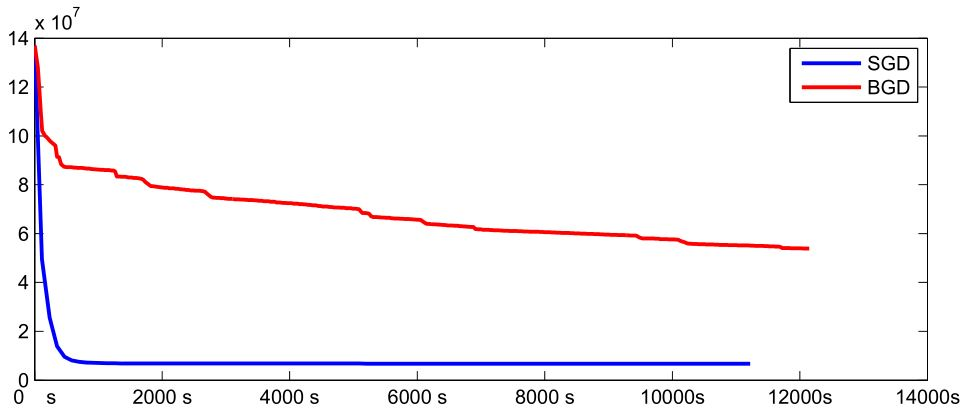
\includegraphics[width=12cm]{BGD.jpg}
    \caption{BGD与SGD性能对比}
    \label{fig-sample}
\end{figure}
可以看出,SGD算法在700s时已接近最优值,速度远比BGD快。因此在这个训练问题上,SGD要比BGD更合适。
\subsection*{2. 转发链长度预测问题定位}
\par 
在解决掉训练时间过长的问题后,我又重新进行了转发链长度预测仿真,但效果相比以前只提高了20$\%$左右。结果如图$2$所示:转发链长度为1的微博数量相差很大。
\begin{figure}[h!]
    \centering
    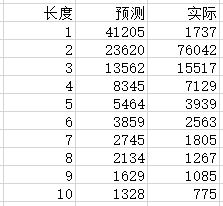
\includegraphics[width=5cm]{size.jpg}
    \caption{转发链长度:预测与实际}
    \label{fig-sample}
\end{figure}
\par
我将所有用户的影响力和敏感度都设为1,即用户只要看到微博,必然转发。在这样的前提下,得到的转发链长度为1的微博数量都有15000条之多,远大于实际的1737。因此问题出在传播网络(Diffusion Network)上。
\par
我们的程序输入是一条条关于用户转发行为的时间序列,需要根据这些数据\textbf{反推出用户间的follower-followee关系}。关于Diffusion Network怎么推导,在论文中作者一笔略过,但给出了数据集对应的Diffusion Network结果数据。但我用这个数据来训练却得到错误的结果。
\par
\textbf{下一步我想研究下Diffusion Network的有关内容},老师您觉得我的下一步方向有没有问题?
\par \rightline{学生王超民,2016年9月11日}

\end{document}
